\documentclass[tikz,border=10pt]{standalone}
% Shared look for every TikZ diagram. Load with % Shared look for every TikZ diagram. Load with % Shared look for every TikZ diagram. Load with \input{../../tools/tikz-style.tex}
\usepackage[T1]{fontenc}
\usepackage{lmodern}
\renewcommand{\sfdefault}{lmr}  % diagrams use the same serif as the text
\usetikzlibrary{arrows.meta, positioning, shapes.geometric, calc, fit, backgrounds}
\definecolor{cblue}{HTML}{4C78A8}
\definecolor{corange}{HTML}{F58518}
\definecolor{cgreen}{HTML}{54A24B}
\definecolor{cred}{HTML}{E45756}
\definecolor{cpurple}{HTML}{B279A2}
\definecolor{cgrey}{HTML}{6B6B6B}
\tikzset{
  every picture/.style={font=\sffamily, line width=1.2pt},
  box/.style={draw=#1, fill=#1!12, rounded corners=4pt, align=center, inner sep=7pt, minimum height=1.1cm},
  box/.default=cgrey,
  arrow/.style={-{Stealth[length=3mm]}, draw=cgrey, line width=1.4pt},
  title/.style={font=\sffamily\bfseries\Large},
  note/.style={font=\sffamily\small, text=cgrey, align=center},
}
\AtBeginDocument{\hyphenpenalty=10000 \exhyphenpenalty=10000}

\usepackage[T1]{fontenc}
\usepackage{lmodern}
\renewcommand{\sfdefault}{lmr}  % diagrams use the same serif as the text
\usetikzlibrary{arrows.meta, positioning, shapes.geometric, calc, fit, backgrounds}
\definecolor{cblue}{HTML}{4C78A8}
\definecolor{corange}{HTML}{F58518}
\definecolor{cgreen}{HTML}{54A24B}
\definecolor{cred}{HTML}{E45756}
\definecolor{cpurple}{HTML}{B279A2}
\definecolor{cgrey}{HTML}{6B6B6B}
\tikzset{
  every picture/.style={font=\sffamily, line width=1.2pt},
  box/.style={draw=#1, fill=#1!12, rounded corners=4pt, align=center, inner sep=7pt, minimum height=1.1cm},
  box/.default=cgrey,
  arrow/.style={-{Stealth[length=3mm]}, draw=cgrey, line width=1.4pt},
  title/.style={font=\sffamily\bfseries\Large},
  note/.style={font=\sffamily\small, text=cgrey, align=center},
}
\AtBeginDocument{\hyphenpenalty=10000 \exhyphenpenalty=10000}

\usepackage[T1]{fontenc}
\usepackage{lmodern}
\renewcommand{\sfdefault}{lmr}  % diagrams use the same serif as the text
\usetikzlibrary{arrows.meta, positioning, shapes.geometric, calc, fit, backgrounds}
\definecolor{cblue}{HTML}{4C78A8}
\definecolor{corange}{HTML}{F58518}
\definecolor{cgreen}{HTML}{54A24B}
\definecolor{cred}{HTML}{E45756}
\definecolor{cpurple}{HTML}{B279A2}
\definecolor{cgrey}{HTML}{6B6B6B}
\tikzset{
  every picture/.style={font=\sffamily, line width=1.2pt},
  box/.style={draw=#1, fill=#1!12, rounded corners=4pt, align=center, inner sep=7pt, minimum height=1.1cm},
  box/.default=cgrey,
  arrow/.style={-{Stealth[length=3mm]}, draw=cgrey, line width=1.4pt},
  title/.style={font=\sffamily\bfseries\Large},
  note/.style={font=\sffamily\small, text=cgrey, align=center},
}
\AtBeginDocument{\hyphenpenalty=10000 \exhyphenpenalty=10000}

\begin{document}
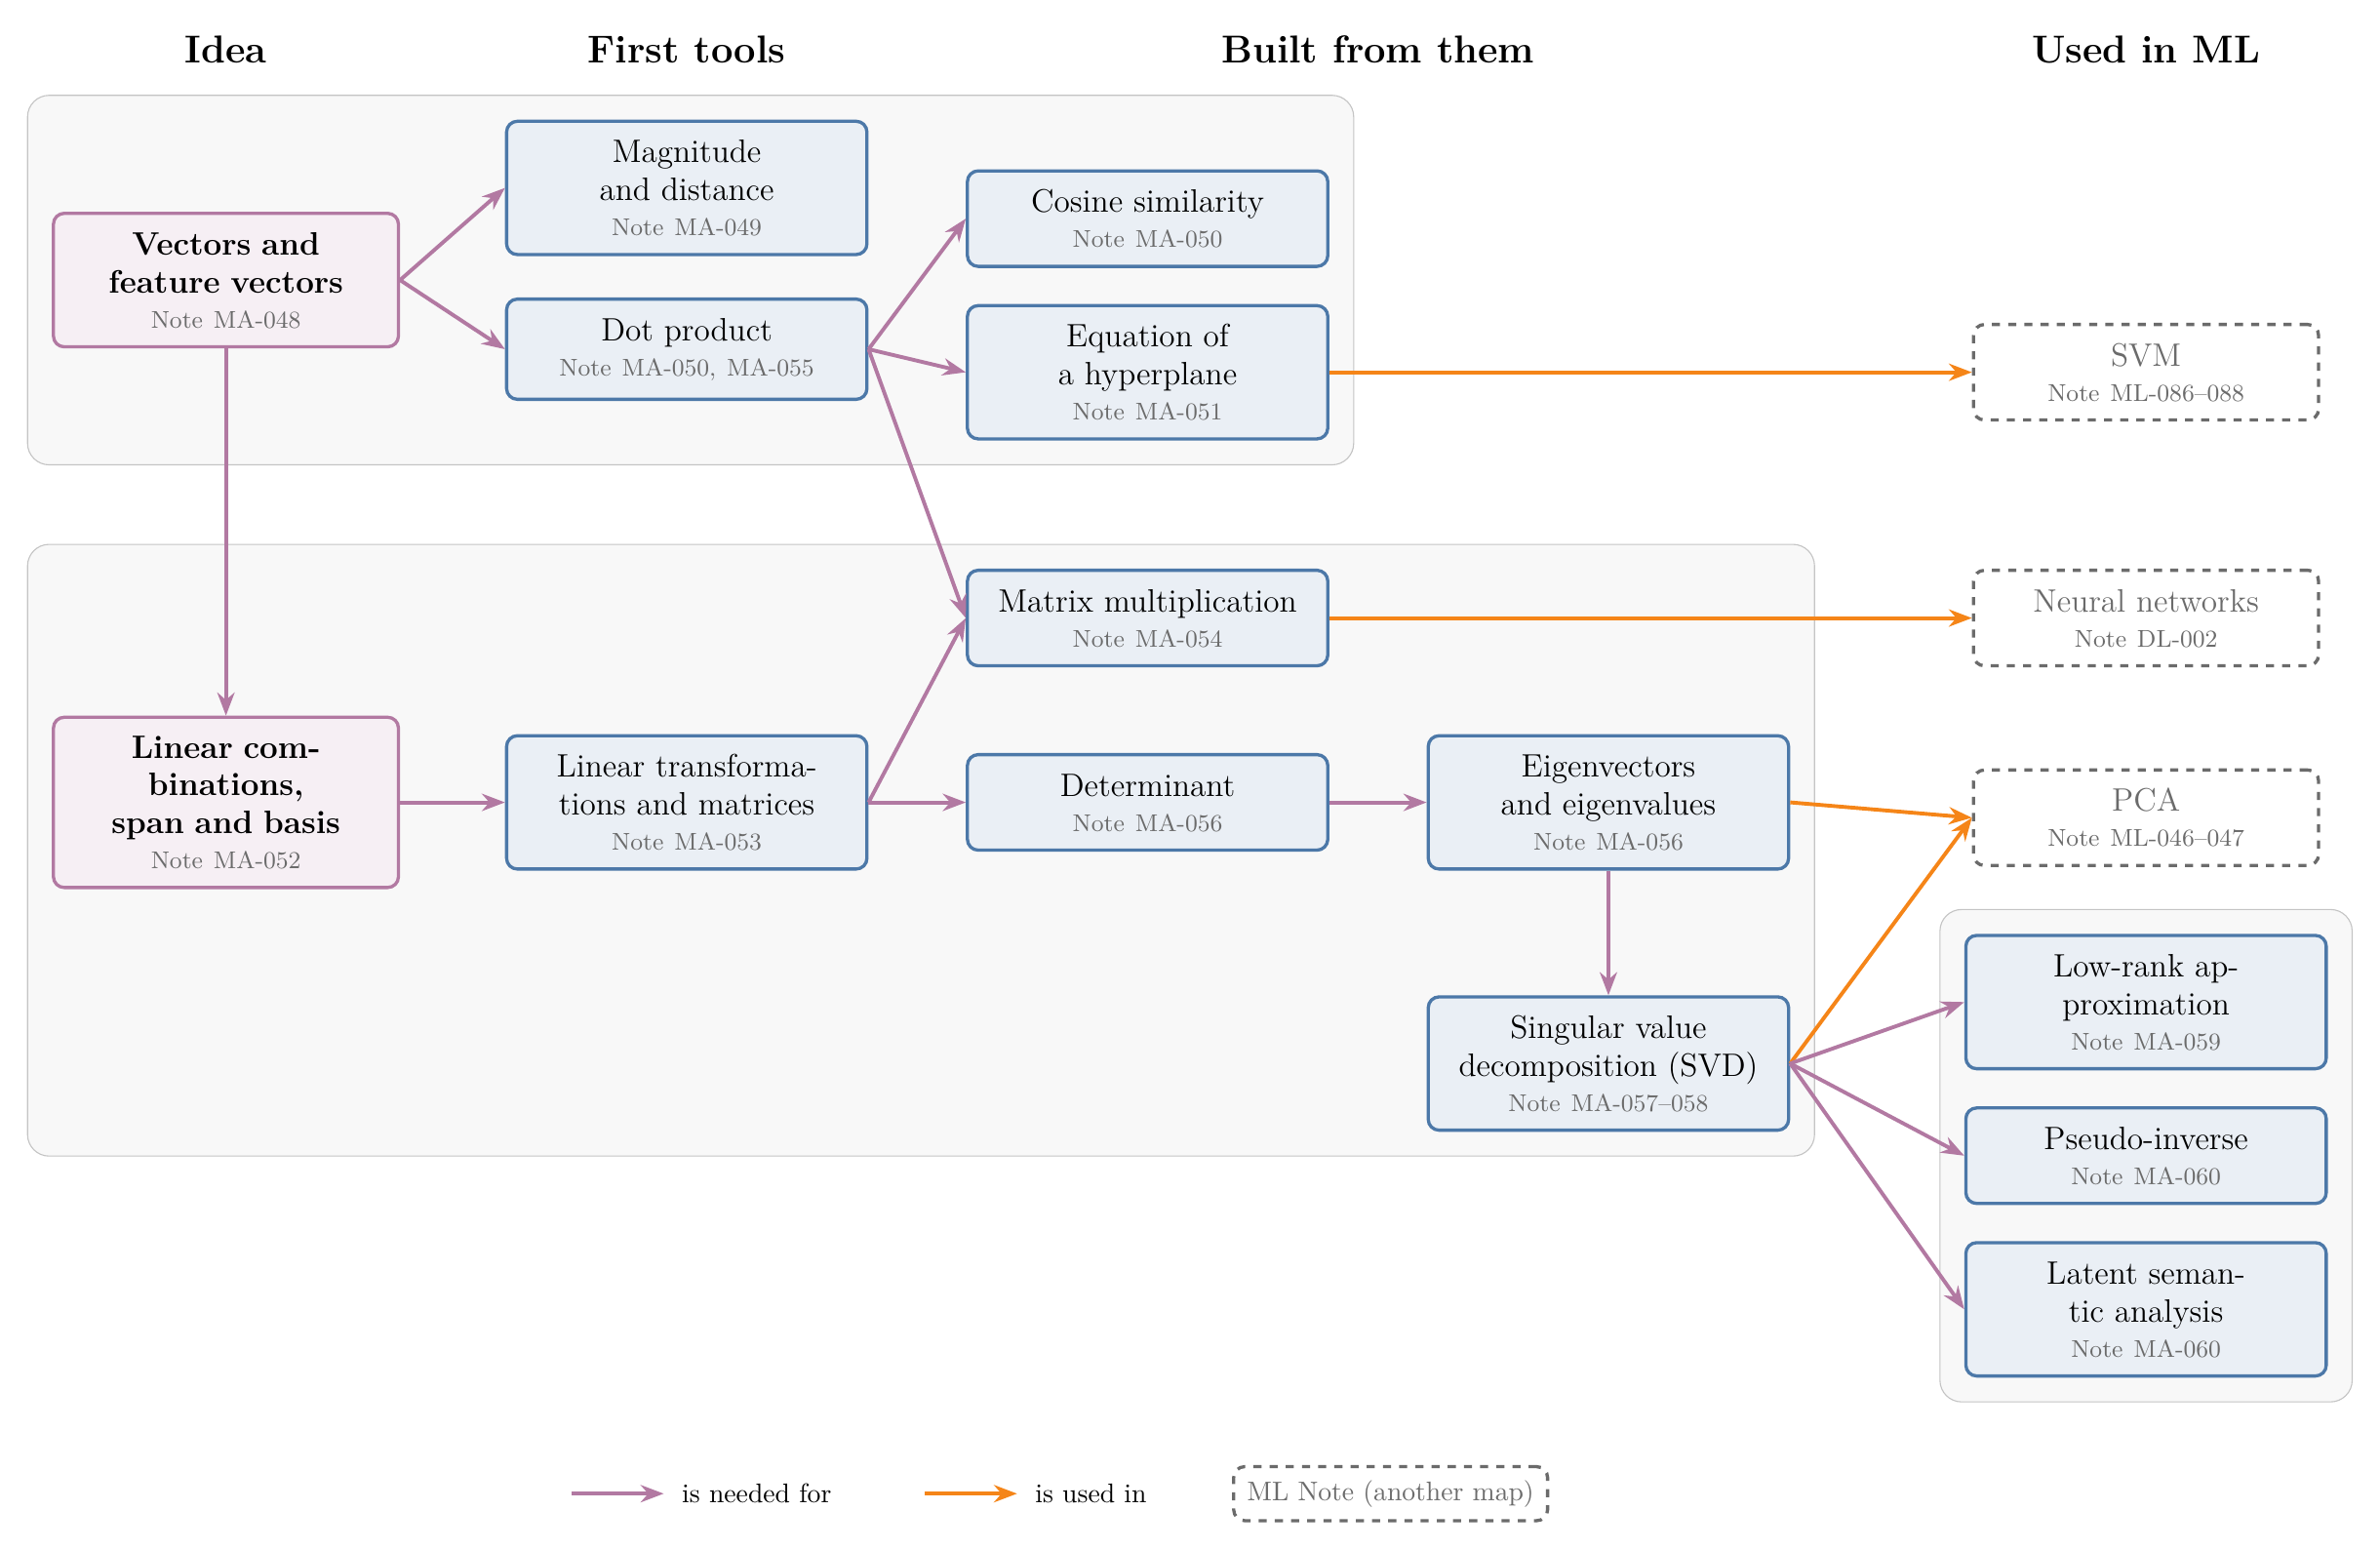
\begin{tikzpicture}[
    every node/.append style={font=\sffamily\large},
    idea/.style={box=cpurple, text width=4.0cm},
    con/.style={box=cblue, text width=4.2cm},
    prev/.style={draw=cgrey, dashed, rounded corners=4pt, align=center, inner sep=7pt, text=cgrey, text width=4.0cm, minimum height=1.1cm},
    group/.style={draw=cgrey!40, fill=cgrey!5, rounded corners=8pt, inner sep=9pt},
    needs/.style={arrow, draw=cpurple},
    used/.style={arrow, draw=corange},
  ]
  \newcommand{\nt}[1]{\\[-1pt]{\small\color{cgrey}Note #1}}
  \node[title] at (0,10.8)  {Idea};
  \node[title] at (6,10.8)  {First tools};
  \node[title] at (15,10.8) {Built from them};
  \node[title] at (25,10.8) {Used in ML};

  % ---- band 1: vectors
  \node[idea] (vec) at (0,7.8)  {\textbf{Vectors and feature vectors}\nt{MA-048}};
  \node[con] (norm) at (6,9.0)  {Magnitude and distance\nt{MA-049}};
  \node[con] (dot)  at (6,6.9)  {Dot product\nt{MA-050, MA-055}};
  \node[con] (cos)  at (12,8.6) {Cosine similarity\nt{MA-050}};
  \node[con] (hyp)  at (12,6.6) {Equation of a hyperplane\nt{MA-051}};

  % ---- band 2: matrices
  \node[idea] (span) at (0,1.0)  {\textbf{Linear combinations, span and basis}\nt{MA-052}};
  \node[con] (lt)   at (6,1.0)   {Linear transformations and matrices\nt{MA-053}};
  \node[con] (mm)   at (12,3.4)  {Matrix multiplication\nt{MA-054}};
  \node[con] (det)  at (12,1.0)  {Determinant\nt{MA-056}};
  \node[con] (eig)  at (18,1.0)  {Eigenvectors and eigenvalues\nt{MA-056}};
  \node[con] (svd)  at (18,-2.4) {Singular value decomposition (SVD)\nt{MA-057--058}};

  % ---- uses
  \node[prev] (svm) at (25,6.6)  {SVM\nt{ML-086--088}};
  \node[prev] (nn)  at (25,3.4)  {Neural networks\nt{DL-002}};
  \node[prev] (pca) at (25,0.8)  {PCA\nt{ML-046--047}};
  \node[con] (lr)   at (25,-1.6) {Low-rank approximation\nt{MA-059}};
  \node[con] (pinv) at (25,-3.6) {Pseudo-inverse\nt{MA-060}};
  \node[con] (lsa)  at (25,-5.6) {Latent semantic analysis\nt{MA-060}};

  \begin{scope}[on background layer]
    \node[group, fit=(vec) (norm) (cos) (hyp) (dot)] {};
    \node[group, fit=(span) (mm) (svd) (eig)] {};
    \node[group, fit=(lr) (pinv) (lsa)] {};
  \end{scope}

  % vectors
  \draw[needs] (vec.east) -- (norm.west);
  \draw[needs] (vec.east) -- (dot.west);
  \draw[needs] (dot.east) -- (cos.west);
  \draw[needs] (dot.east) -- (hyp.west);
  \draw[used]  (hyp.east) -- (svm.west);
  \draw[needs] (vec.south) -- (span.north);

  % matrices
  \draw[needs] (span.east) -- (lt.west);
  \draw[needs] (lt.east) -- (mm.west);
  \draw[needs] (dot.east) -- (mm.west);
  \draw[needs] (lt.east) -- (det.west);
  \draw[needs] (det.east) -- (eig.west);
  \draw[needs] (eig.south) -- (svd.north);
  \draw[used]  (mm.east) -- (nn.west);
  \draw[used]  (eig.east) -- (pca.west);
  \draw[used]  (svd.east) -- (pca.west);
  \foreach \u in {lr, pinv, lsa} \draw[needs] (svd.east) -- (\u.west);

  % legend
  \begin{scope}[shift={(4.5,-8.0)}, every node/.style={font=\sffamily, anchor=west}]
    \draw[needs] (0,0) -- (1.2,0);     \node at (1.3,0) {is needed for};
    \draw[used] (4.6,0) -- (5.8,0);    \node at (5.9,0) {is used in};
    \node[draw=cgrey, dashed, rounded corners=4pt, inner sep=5pt, text=cgrey, anchor=west] at (8.6,0) {ML Note (another map)};
  \end{scope}
\end{tikzpicture}
\end{document}
